Ce rapport d'état de l'art fournira une introduction du paysage de la recherche sur la mesure de l'impact, la théorie du changement, les systèmes de suivi et d'évaluation dans le contexte des meta-organisations. En s'appuyabt dans notre cas sur les alliances d'universités. 

Alors que nous nous concentrons sur différents axes autour de notre cadre potentiel, nous avons étudié notre problématique à travers différents prismes et angles. 
Commençons par définir l'impact et la méthodologie utilisée. Nous allons utiliser la définition suivante du Comité d'aide au développement (CAD) de l'Organisation de coopération et de développement économiques (OCDE) :

« Effets à long terme, positifs et négatifs, directs et indirects, intentionnels et non intentionnels produits par une intervention de développement »\cite{oecd_quality_2010}

\begin{figure}
    \centering
    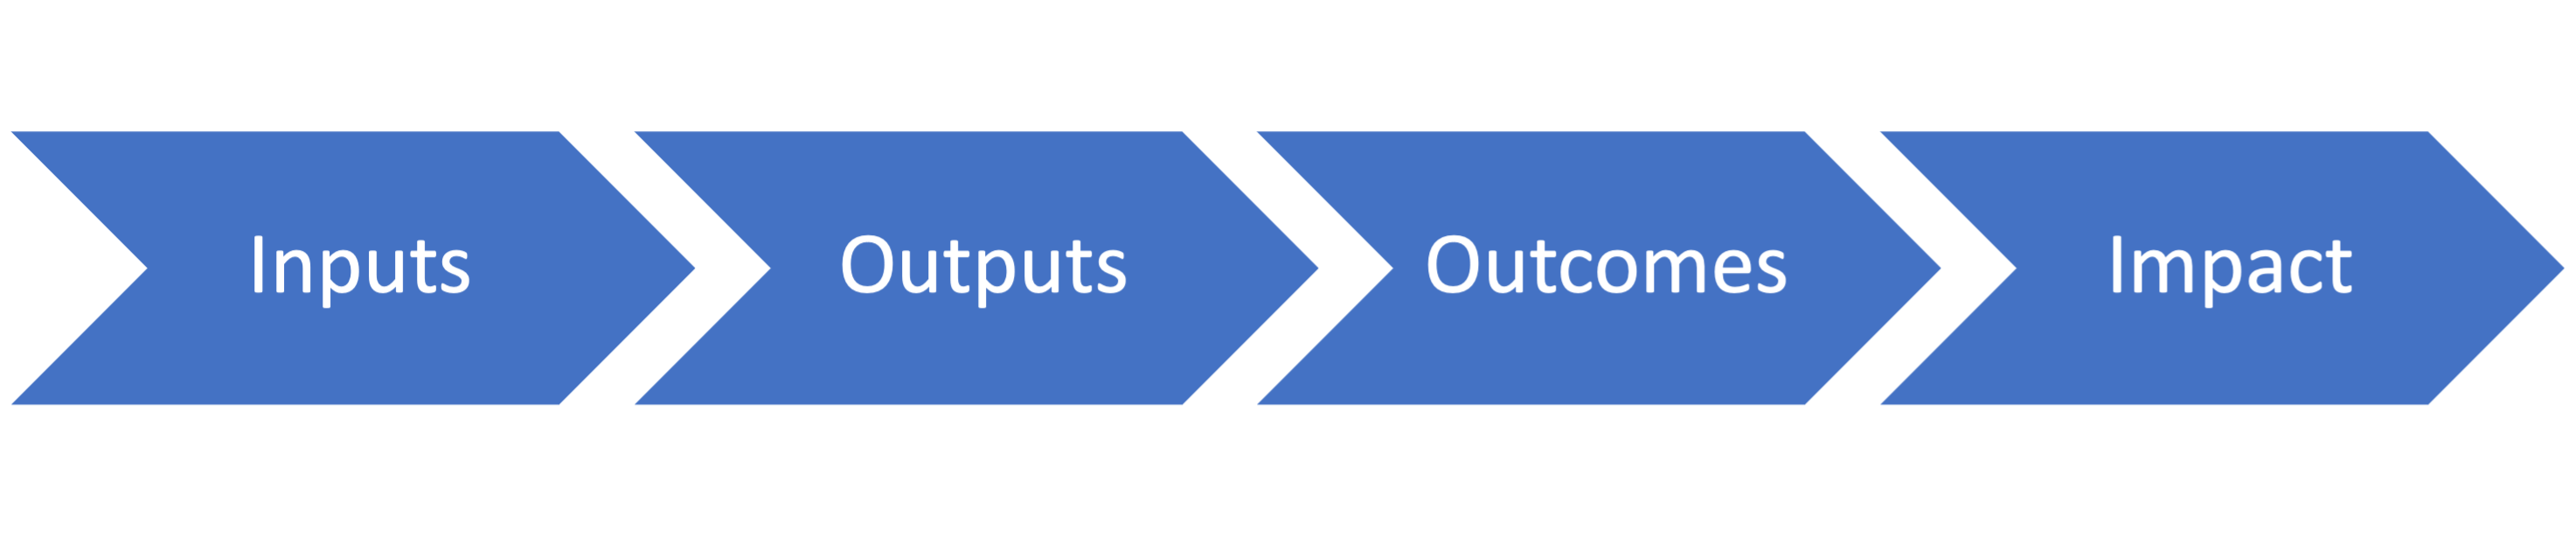
\includegraphics[width=1\linewidth]{Modele_Latex_CNRIUT2025//images/impact-chain.png}
    \caption{Chaîne de mesure d’impac\cite{stein_understanding_2012}}
    \label{fig:impact-chain}
\end{figure}
Maintenant, en s'appuyant sur la figure \ref{fig:impact-chain}, nous allons définir ses termes.
\begin{itemize}
    \item Inputs: Représentent les ressources et les matériaux nécessaires pour lancer un projet ou un programme.
    \item Outputs: Résultats directs et immédiats des activités, souvent quantifiables et mesurables.
    \item Outcomes: Indiquent les réalisations initiales résultant des sorties et des activités, contribuant aux objectifs du projet.
    \item Impact: Représente les effets à long terme et les changements plus larges qui se produisent en raison du projet, influençant les parties prenantes et la communauté.
\end{itemize}

Étant donné que le point suivant a été largement accepté et reconnu, nous nous référons aux alliances d'universités comme des meta-organisation dans cet article. Définies comme « Des organisations dont les membres sont d'autres organisations »\cite{ahrne_organizations_2005}. Cependant, il est intéressant de questionner la validité de la théorie du changement, de la méthodologie d'impact et bien plus encore dans ce contexte précis.

Il est admis dans le domaine que la théorie du changement (ToC) répond à la question : « Comment se produit le changement réussi ? ». Dans cet ordre, la définition et le but semblent clairs. Cependant, en fouillant dans la littérature, vous pouvez tomber sur de nombreuses théories différentes. Ces théories se contredisent parfois et il est clair que la ToC peut sembler être un mot d'ordre de développement plutôt qu'une signification tangible\cite{stein_understanding_2012}. 

Enfin, notre solution proposée d'un système de suivi et d'évaluation de l'impact par le biais d'un entrepôt de données alimenté par une base de connaissances nécessite quelques définitions. Un système de suivi et d'évaluation (S\&E) utilise deux termes étroitement liés. La \textbf{surveillance} est l'acte de suivre fréquemment et de rapporter des informations prioritaires sur une intervention. Alors que \textbf{l'évaluation} fait référence à des analyses et des études discrètes pour produire un jugement global et une signification d'une intervention, ainsi que pour décrire les relations possibles entre les éléments.